% !TEX root = collhdl_ICRA_17.tex

\section{Evaluation and Case Studies}
\label{sec:simu}

\subsection{General Simulation Setup}
\label{sec:setup}
The simulative setup is as follows.
We apply our collision detection, isolation and identification algorithm in simulation to an \emph{Atlas} robot consisting of cylinders and cuboids as collision geometry from \cite{DRCSim}.
We assume perfect measurements of the generalized joint forces and the force/torque sensors unless stated differently, meaning all sensors measure the true value without noise or delay.
Force/torque sensors are placed at the end-effectors (feet and hands), before the first arm and leg joints and at the upper torso after the three back joints (see Fig.~\ref{fig:coll_singlecontact_overview}).
Furthermore, all acting external forces comply with the assumption of a pushing force and the line of action of the forces is chosen such that it does not intersect with any other collision body before the contact point.
The robot pose (see Fig.~\ref{fig:coll_singlecontact_overview}) has been chosen in such a way that the whole body Jacobian has full rank.
The robot is modeled in free space, meaning there are no other external forces acting on the robot than the collision forces.
The simulation is done on a standard Core i7-3770 PC and the algorithm is run as compiled Matlab functions.
With the current implementation, the majority of the runtime for all contact cases is spent on the not yet optimized intersection algorithm.

\subsection{Ideal Analysis of Single Contacts}
\label{sec:eval_single_static}
We compare the ideal performance of the isolation based on estimated generalized external forces $\hat{\bm{\tau}}_\epsilon$ only (Sec.~\ref{sec:isolation}) to the isolation based only on force/torque sensor measurements $\hat{\bm{\mathcal{F}}}_{\mathrm{ext},S}$ (from (\ref{eqn:cmp})) for a single contact.
Dynamic effects due to the observer and load compensation are neglected for sake of clarity.
The contact points are distributed randomly and equally over the robot surface.
Figure~\ref{fig:coll_singlecontact_overview} depicts the results of the isolation procedures with some representative samples of the 3000 tested points.
With both methods, the contact points are isolated correctly up to rounding errors, if possible.
The contacts at the pelvis cannot be seen by any force/torque sensor and can therefore only be isolated with the generalized external forces acting on the base.
The maximum and mean execution times for the isolation of the one contact in this experiment were 0.67~ms and 0.25~ms using force/torque sensors as well as 0.57~ms and 0.17~ms using joint torque measurements only.
\begin{figure}
\begin{center}
\begin{overpic}{figures/collest_single_allresults_nosim/coll_est_sc_all_nosim}
\put(82,54){\line(-1,-2){7}}
\put(56,11){\line(1,2){11}}
\put(67,35){F/T sensor}
\end{overpic}
\end{center}
\caption{Distribution of true ($\bm{r}_\mathrm{C}$) and estimated contact locations using two different methods.
The points $\hat{\bm{r}}_C(\hat{\bm{\tau}}_\epsilon)$ are isolated using only generalized external forces and the points $\hat{\bm{r}}_C(\hat{\bm{\mathcal{F}}}_{\mathrm{ext,S}})$ are isolated using the force/torque sensor measurements only.
For the pelvis (base link) and first torso links, no force measurement is available. Therefore contact points at these links cannot be found with the latter method.
All overlying points are identical up to rounding errors.}
\vspace*{-0.8cm}
\label{fig:coll_singlecontact_overview}
\end{figure}

\subsection{Ideal Analysis of Multiple Contacts}
\label{sec:eval_multi_static}
In the following, we analyze multiple contacts of the type specified in Sec.~\ref{sec:eval_single_static}.

\subsubsection{Two Contacts at different links}

The considered contact points are located at different links, since two contacts at the same link cannot be located in our setup. In order to be able to do so, one would need two force/torque sensors in the same link.
5000 random combinations were examined.

The algorithm using generalized forces is able to isolate all two contact point coordinates up to rounding errors if the rank of the Jacobian in (\ref{eqn:force_identification}) is sufficiently high, e.g. $\mathrm{rank}(\bm{J})=12$ for $N_\mathrm{C}=2$ contact points.
Figure~\ref{fig:coll_multicontact_rankJ} shows the success of the isolation for different contact links, which is equivalent to the plot of the rank deficit
\begin{equation}
RD=6N_\mathrm{C}-\mathrm{rank}(\bm{J}).
\label{eqn:rank_deficit}
\end{equation}
For example, a contact at the pelvis (torso chain link 1) and another contact at the left lower leg (left leg chain link 4) does only produce 10 nonzero columns in the stacked Jacobian and the isolation fails (see corresponding entry in Fig.~\ref{fig:coll_multicontact_rankJ}).
If instead the foot on the left leg chain (link 6) is in contact, then 12 nonzero columns exist and the isolation succeeds.

For a rank deficit, the isolation method minimizes the Cartesian error of the stacked identified wrenches and finds contact points on the entire following kinematic chain. 
The distribution of errors for different ranks of the Jacobian is shown in Fig.~\ref{fig:hist_rank_err_2coll}.
An error $\leq$ 25~cm occurs in about 80\% of the cases with the joint configuration from Fig.~\ref{fig:coll_singlecontact_overview}.
Please note that in case of a rank deficit, the algorithm may accidentally estimate an additional contact point, which would be located close to the base.
The error is then calculated between the real contact points and the ones estimated in the same kinematic chain.
The maximum and mean execution times for the isolation in this experiment were 0.75~ms and 0.28~ms using force/torque sensors as well as 31.8~ms and 3.6~ms using joint torque measurements only.

\begin{figure}
\begin{center}
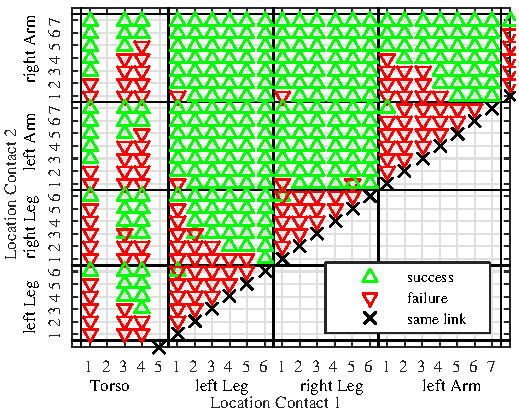
\includegraphics[width=\columnwidth]{figures/collest_multi_stat_2coll_rankmat/rankmat_fig_2coll_Modus2}
\end{center}\vspace*{-0.3cm}
\caption{Overview of success and failure for the isolation of two simultaneous contacts.
The $x$-axis gives the first contact link and the $y$-axis the second one.
The second and the last body of the torso chain have no collision body in the model, the according columns are therefore left empty.
A green upward triangle marks the successful isolation of both contact points for the given combination.
A red downward triangle marks a combination for which it was impossible to isolate the contacts correctly due to rank loss of the combined Jacobian in (\ref{eqn:multi_iso}).
In some fields, green and red triangles are plotted meaning that for this combination, the isolation was only partly correct.
For the combination of the fifth link in the right leg and the first link of the right arm, this is due to the fact, that for some contacts, the joint torque threshold for the last joint is not exceeded and the algorithm is therefore started with a loss of rank in the Jacobian.
However, when reducing the joint torque threshold or starting the algorithm with the correct contact links, this could not be observed anymore.
In the other cases, the contact point was estimated correctly by accident with a rank deficient Jacobian.
Overall 5000 combinations were tested.}\vspace*{-0.5cm}
\label{fig:coll_multicontact_rankJ}
\end{figure}

\begin{figure}
\vspace*{-0cm}
\begin{center}
% Um die Prozentangaben für Overpic zu generieren: Skript histogram_error_rank.m im Bildordner ausführen und aus Textausgaben entnehmen.
\begin{overpic}{figures/collest_multi_stat_2coll_error_rank/hist_rank_err_2coll}
\put(50,78){\line(2,0){10}}
\put(63,76){$100\%$}

\put(49,47){\line(2,3){8}}
\put(56,61){$34\%$}

\put(43,35){\line(1,1){15}}
\put(55,52){$21\%$}

\put(55,36){\line(2,1){7}}
\put(55,40){$11\%$}

\put(68,17){\line(1,1){15}}
\put(80,34){$2\%$}
\end{overpic}
\end{center}
\caption{Histogram of the maximum point estimation error for two contacts with different random contact configurations. Read: ``34\% of the results for $\mathrm{rank}(\bm{J})=11$ lie between 15 and 25~cm.''}
\label{fig:hist_rank_err_2coll}
\vspace*{-0.3cm}
\end{figure}

\subsubsection{Contacts at four end-effectors}

For the considered 30~DoF humanoid, it is possible to detect and isolate up to $N_\mathrm{C}=5$ contacts, if the rank deficit $RD$ is zero.
This is the case for four contacts at the end-effectors of every kinematic chain (feet, hands) and an additional contact located at the torso or first shoulder link, which is the typical manipulation scenario from Fig~\ref{fig:manip}.
The distribution of position errors for this case are depicted in Fig.~\ref{fig:error_rank_manipcoll} with markers for different rank deficits $RD$.

Without rank deficit, the isolation is successful in all but 5 of the 5000 examined points, where there was no rank deficit.
The errors occur in situations, where the joint torque threshold for the last joint in at least one chain is not exceeded.
This leads to a Jacobian with rank-deficit for the first iteration step of the algorithm, making it in a few cases impossible to find the correct contact link.
However, if the threshold is reduced to $10^{-5}$~N or Nm (for all  $\lVert\bm{f}_{\mathrm{ext},i}\rVert<1$), or the algorithm is started with perfect information about the contact links, no errors are observed.
The maximum and mean execution times for the isolation in this experiment were 0.92~ms and 0.52~ms using force/torque sensors as well as 43.2~ms and 11.0~ms using joint torque measurements only.

\begin{figure*}
\begin{center}
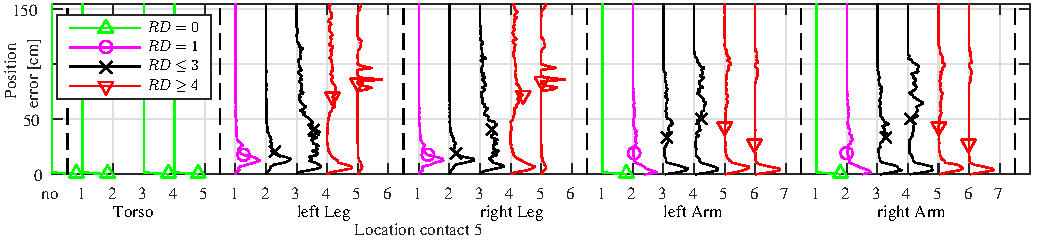
\includegraphics{figures/collest_multi_stat_manipcoll_error/error_rank_manipcoll_hist_breit}
\end{center}\vspace*{-0.4cm}
\caption{Distribution of the isolation position error based on joint torques only with contacts at all end-effectors for different rank deficits $RD$ of the Jacobian.
The position error distributions are drawn over the location for a fifth contact.
The fifth contact location can be none (only four contacts) or any of the links, which are not an end-effector link.
Therefore the four columns of the end-effectors are left empty.
The columns of the second and the last torso chain link are left empty, because their model does not have any contact bodies, making it impossible to place contacts at these links.
Markers in the lines denote the mean errors of all contact points including this link.
The distribution lines are normalized to the highest corresponding value of the distribution.}\vspace*{-0.7cm}
\label{fig:error_rank_manipcoll}
\end{figure*}

\subsubsection{Benefits of additional force/torque sensors}

The results show the benefits of supplementary force/torque sensors, see Table~\ref{tab:sensor_benefits}.
Without force/torque sensors, up to five contacts can be detected, isolated and identified correctly under certain conditions.
With force/torque sensors in the distal links, at least the generalized external manipulation and locomotion forces can be found and further contacts can be isolated by additional force/torque sensors (max. one per sensor) or the first method (up to 5 in theory).
%
\begin{table}
\caption{Possibilities of collision detection, isolation and identification with different numbers of force/torque sensors in the kinematic tree. The sensors are meant to be added up down the lines of the table.}\label{tab:sensor_benefits}
\begin{tabular}{|p{2.8cm}|p{5cm}|}
\hline
sensors & possibilities\\\hline
only joint torque and base movement sensors & identify ground contact and manipulation contacts, detect single collision, isolate and identify single collision under certain conditions (see Fig.~\ref{fig:error_rank_manipcoll})\\\hline
distal force/torque sensors & full elimination of ground contact and manipulation forces, detection isolation and identification of single collisions, multiple collisions can be detected, isolated and identified in many cases\\\hline
additional force/torque sensors in the kinematic chains & detect isolate and identify one additional contact wrench per additional sensor\\\hline
\end{tabular}\vspace*{-0.3cm}
\end{table}

\subsection{Time Series Analysis of a Single Contact}
The influence of the observer dynamics on the isolation and identification is investigated by using generalized external forces including observer dynamics.
The external force acts over a sinus half wave with an amplitude of one and a cycle time of 40~ms.
The observer is run at a sample frequency of 1000~Hz and $K_O=500$ as suggested in \cite{Haddadin2014}.
In this simulation, the observer error and the error in acceleration estimation for the force/torque sensor compensation are assumed to follow the dynamics presented in (\ref{eqn:obs_dynamic}) and (\ref{eqn:qDD_dyn}) respectively.
%
\begin{figure}
\begin{center}
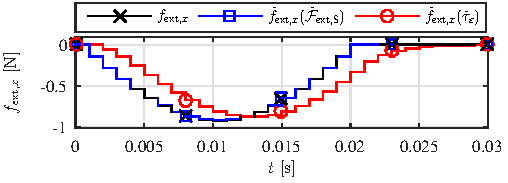
\includegraphics{figures/colltest_single_filter/colltest_single_filter_f}
\end{center}\vspace*{-0.4cm}
\caption{The $x$-component of the external force $\bm{f}_\mathrm{ext}$, the external force estimated with force/torque sensors  $\hat{\bm{f}}_{\mathrm{ext}}(\hat{\bm{\mathcal{F}}}_{\mathrm{ext,S}})$ according to (\ref{eqn:cmp}) and (\ref{eqn:cmp_ext_vorher}) as well as the external force estimated with the observed generalized forces $\hat{\bm{f}}_{\mathrm{ext}}(\hat{\tau}_\epsilon)$ according to (\ref{eqn:force_identification}) is depicted over time for a collision of  20~ms.
When using the generalized forces for identification, the estimated external force is a first order filtered version of the real force with time constant $K_O^{-1}$.
Using compensated force/torque sensors, the estimated force follows the real force without any delay.}\vspace*{-0.6cm}
\label{fig:coll_singlecontact_filter}
\end{figure}
%
With both methods described before, the contact point is isolated correctly up to numerical errors.
If the observed generalized joint forces are used for isolation, there is a delay of one time step, as the filtered generalized forces are still zero for the first time step of the collision.

Fig.~\ref{fig:coll_singlecontact_filter} shows the external forces over the collision time and the forces identified with and without the use of force/torque sensors.
It can be seen that if no force/torque sensors are used, the contact force is estimated with a delay of approximately 3~ms.
It has to be noted, that the collision will be seen about 10~ms longer with the observer dynamics taken into account.
This timespan depends on the thresholds for the generalized external forces, which was here chosen to be 0.001~N or 0.001~Nm, respectively and the filter frequency $1/K_O$.
Furthermore, when using force/torque sensors, smaller delay but larger error in the estimated external force can be observed.
As the error of $\hat{\ddot{\bm{q}}}$ is driven by $\bm{\tau}_\mathrm{ext}$ and $\bm{M}(\bm{q})$ is nearly constant for the robot at standstill, the contact point can still be estimated correctly with the compensated force/torque sensor.

